\chapter{Open Problems}
\label{ch:future_work}

	\subsection{Parallel processing (CPU)}
	\label{ssect:parallel_cpu}
	
	
	\subsection{Parallel processing (GPU)}
	\label{ssect:parallel_gpu}


\section{Future Work}
\label{sect:future_challenges}

Considering GRAPHINIUS an arbitrarily extendable computing platform (which uses graphs as underlying, universal data structures), there are many possibilities to build upon this work, ranging from small improvements to the introduction of fundamentally new infrastructure, transcending the use of contemporary graph libraries. 

The use of a centralized, Web based graphical workflow system will prove especially useful in exploiting and propagates the experience of individual users, as it bundles not only data, but also the settings and results of all experiments conducted on that platform.


\subsection{Graph generators (graph types)}
\label{ssect:graph_gen}


\subsection{Graph classifiers}
\label{ssect:graph_class}


\subsection{JSVM based grid computing}
\label{ssect:jsvm_grid}


\subsection{General processing / ML pipelines}
\label{ssect:pipelines}

As existing stacks indicate, there are several possible levels of pipelines which can be sorted by increasing homogeneity amongst their stages as well as decreasing technical demands on their users:

\begin{itemize}
	\item Level 0: Writing all of the pipeline manually. As every combination of technologies are usable, this approach gives the most flexibility but is hard to maintain and almost impossible to reproduce. As \citep{MLTechnicalDebt} perfectly states: ``Using self-contained solutions often results in a glue code system design pattern, in which a massive amount of supporting code is written to get data into and out of general-purpose packages.''
	
	\item Level 1: Automated, but self designed and coded. This entails the usage of tools like Unix Make, which is language agnostic and therefore supports any number of technologies as long as they are executable from a Shell. Apart from slightly better decoupling, same problems as Level 0.
	
	\item Level 2: Establishing a common understanding of the components and structure of a pipeline while still using individual technologies. Such a common standard exists in the form of PMML - the Predictive Model Markup Language. PMML defines stages of pipelines as well as their inputs, parameter types and ranges, the output format etc. Thus, developers can use their favorite technologies in the development phase while PMML consuming tools then produce familiar code (Hadoop, Spark, ..).
	
	\item Level 3: Language specific libraries exposing an API to conveniently assemble a pipeline. Such libraries have been released by projects like scikit-learn or Apache Spark. While currently becoming popular, APIs still restrict the creation of data applications to experts capable of coding.
	
	\item Level 4: The use of a custom DSL would widen the ability to create complex data pipelines to any kind of domain expert. Similar in nature to SQL, it is able to either compile itself into code or an intermediate representation like PMML.
	
	\item Level 5: A fully integrated data analysis platform that offers intuitive, visual pipeline assembly. Ideally, tools for reporting, reproduction and collaboration would also be included. In addition, the platform could offer experts the means to write stages themselves via an online code editor. OGMA is designed to be such a platform.
\end{itemize}


\subsection{Heterogeneous data linkage}
\label{ssect:heterogeneous_data}

Many research fields comprise several sub-problems which are amenable to different machine learning approaches and feature their own, distinctive input data sets. Coming from various, different data sets featuring their distinct attribute domains, they probably are - via their time-, space- or other dimensions, interlinkable with one another. Usually, studies are only concerned about using a single one of those data sources and applying different methods to it. However, a more holistic approach would be to fuse those data sets along one or more dimensions (or any other meaningful ruleset) in order to achieve a richer representation of the underlying problem. A resulting data-set might take the form of a graph structure, in which individual entities from the originating sets are linked by meaningful connection rules, which in themselves will have to be learned. 

%For example, \cite{thebook} introduced the concept of authority ranking for heterogeneous networks, where the impact is transferred along edges to simultaneously rank nodes of different types.

\subsection{Meta machine learning}
\label{ssect:meta_ml}

Meta-learning applies learning algorithms on data collected about machine learning experiments. As one of the first papers regarding this topic, \citep{Rice1975} defined the "Algorithm Selection Problem", which was first recognized as a meta learning problem by the machine learning community. He describes five spaces in which the Algorithm Selection Problem plays out:

\begin{itemize}
	\item \textbf{The problem space}: This is the set of all possible input problems (datasets + desired result class).
	
	\item \textbf{The feature space}: Features of a specific problem or family of problems. In dermatological imaging those would be defined by the imaging method (laser-scan vs. stanza), the scale of the objects to be detected (single cells vs nevi) etc.
	
	\item \textbf{The algorithm space}: The set of all algorithms suitable for the specific problem (features) to be worked on.
	
	\item \textbf{The performance measures} (the metric space): The set of possible measurements that could describe the quality of a solution (runtime performance, accuracy, ..).
	
	\item \textbf{The criteria space}: The weighing of different performance measures considered for a particular solution.
\end{itemize}


In most scenarios concerning Graphinius we will be concerned with the selection of workflow components and their parameters based on the nature of the specific area of application, the tackled problems, their features, available algorithms, preprocessing methods, parameters as well as performance measures.

\subsection{Hyper heuristics}
\label{ssect:hyper_heuristics}

Hyper heuristics are a way of selecting or configuring algorithms by searching a space of lower level heuristics instead of searching the solution (parameter) space itself. Hyper heuristics are different from meta learning in that they work independently of the problem domain and therefore promise to be generally applicable; the challenges lie in producing algorithms that do not need to be optimal, but rather good-enough, soon-enough, cheap-enough \citep{Burke:2003:Hyperheuristics}.

Although many research fields in themselves are not broad enough to be a suitable proving ground for hyper heuristic research, the Graphinius platform will provide us with meta-data about experiments in many diverse areas. We fully agree with \cite{Burke2013} who concludes that there is still little interaction between research communities, a problem whose solution could lead to the extension of algorithms to both new problem domains and new methodologies through cross-fertilization of ideas.


\subsection{Meta ML / heuristics database}
\label{ssect:heuristics}

The greatest advantage of using Meta ML in combination with a centralized, Web based workflow system lies in the fact that users may profit from their colleagues' meta data by building up a collective Meta ML database: input data plus algorithm parameters plus success metrics.


\subsection{Algorithmic recommender}
\label{ssect:algo_recommender}


\subsection{Interactive Machine Learning}
\label{ssect:fut_iml}

\begin{figure}[ht]
	\begin{center}
		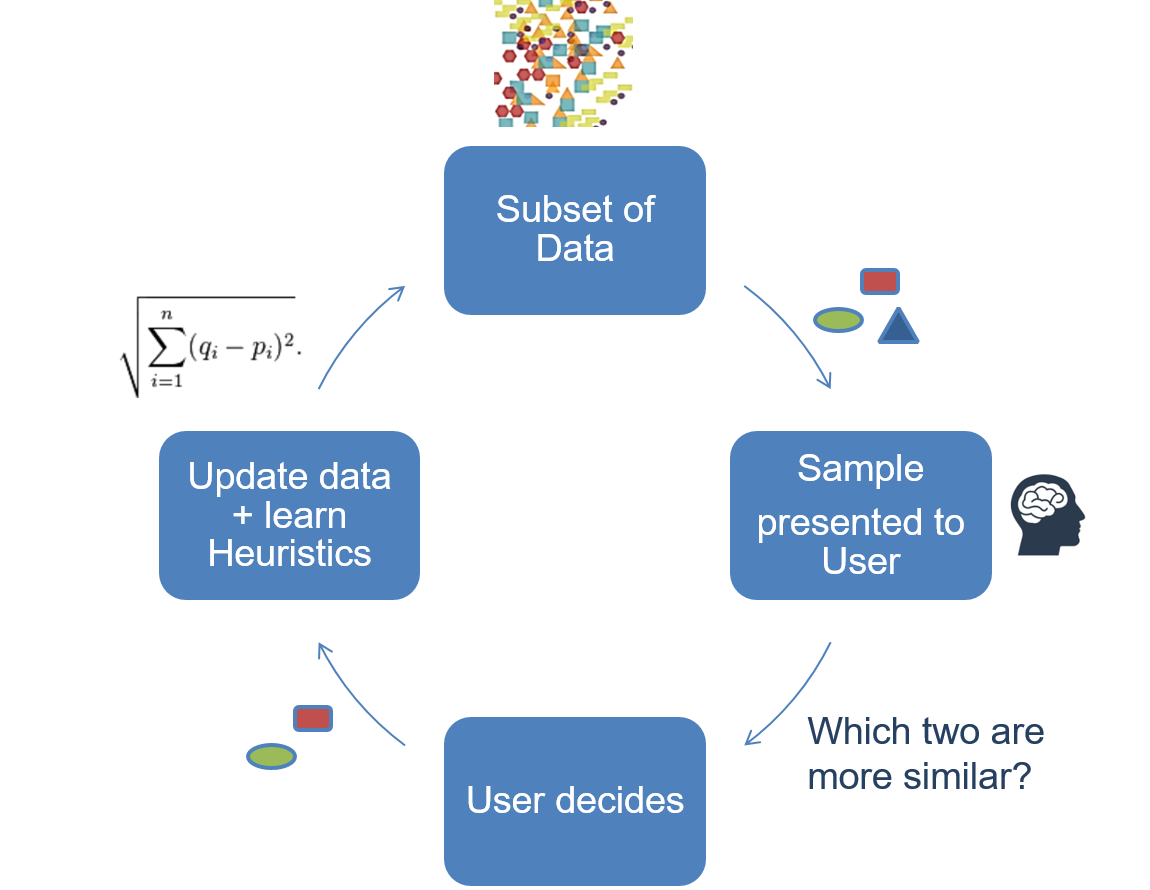
\includegraphics[width=1\textwidth]{figures/anonym/anonIML}
		\caption{Anonymization augmented by IML (human in the loop)}
		\label{fig:anonIML}
	\end{center}
\end{figure}
